% Chapter 3. The three shapes of Streamable HTTP traffic.
\documentclass[tikz,border=6pt]{standalone}
% Shared look for every TikZ figure in the book.
% Colours match book/preamble.tex exactly. Change both or neither.

\usepackage{tikz}
\usepackage{xcolor}
\usepackage{amsmath}
\IfFileExists{libertinus.sty}{\usepackage[mono=false]{libertinus}}{}
\IfFileExists{inconsolata.sty}{\usepackage[varqu,varl,scaled=0.95]{inconsolata}}{}

\usetikzlibrary{
  arrows.meta, positioning, calc, fit, backgrounds, shapes.geometric,
  shapes.misc, decorations.pathreplacing, decorations.pathmorphing,
  patterns, chains, matrix, shadows.blur
}

\definecolor{ink}{HTML}{15181D}
\definecolor{muted}{HTML}{5B6472}
\definecolor{rule}{HTML}{C9CED6}
\definecolor{wash}{HTML}{F4F5F7}
\definecolor{accent}{HTML}{0F5C8C}
\definecolor{accentsoft}{HTML}{E7F0F6}
\definecolor{warm}{HTML}{B4531A}
\definecolor{warmsoft}{HTML}{FBF0E7}
\definecolor{good}{HTML}{2C6E49}
\definecolor{goodsoft}{HTML}{E9F2EC}
\definecolor{danger}{HTML}{9B2226}
\definecolor{dangersoft}{HTML}{FAECEC}

\tikzset{
  font=\sffamily\small,
  >={Stealth[length=5pt, width=4pt]},
  %
  box/.style={
    draw=rule, line width=0.8pt, fill=wash, rounded corners=2pt,
    inner sep=7pt, align=center, text=ink, minimum height=9mm,
  },
  boxa/.style={box, draw=accent, fill=accentsoft},
  boxg/.style={box, draw=good,   fill=goodsoft},
  boxw/.style={box, draw=warm,   fill=warmsoft},
  boxd/.style={box, draw=danger, fill=dangersoft},
  %
  lane/.style={draw=rule, line width=0.7pt, fill=white, rounded corners=2pt,
               inner sep=6pt, align=center, minimum width=26mm},
  %
  flow/.style={draw=accent, line width=1.0pt, ->},
  flowback/.style={flow, densely dashed},
  flowmuted/.style={draw=muted, line width=0.8pt, ->},
  lifeline/.style={draw=rule, line width=0.7pt, densely dotted},
  %
  lbl/.style={font=\sffamily\scriptsize, text=muted, inner sep=2pt},
  lblink/.style={font=\sffamily\scriptsize, text=ink, inner sep=2pt},
  tag/.style={font=\ttfamily\scriptsize, text=accent, inner sep=2pt,
              fill=white, inner xsep=3pt},
  note/.style={font=\sffamily\scriptsize\itshape, text=muted, align=left},
  %
  band/.style={draw=none, rounded corners=1pt},
  tick/.style={draw=muted, line width=0.6pt},
}

% A horizontal timeline bar segment: \barseg{x0}{x1}{y}{colour}{label}
\newcommand{\barseg}[5]{%
  \fill[#4, rounded corners=1pt] (#1,#3-0.16) rectangle (#2,#3+0.16);
  \node[lbl, text=white, font=\sffamily\scriptsize\bfseries]
       at ({(#1+#2)/2},#3) {#5};
}

\begin{document}
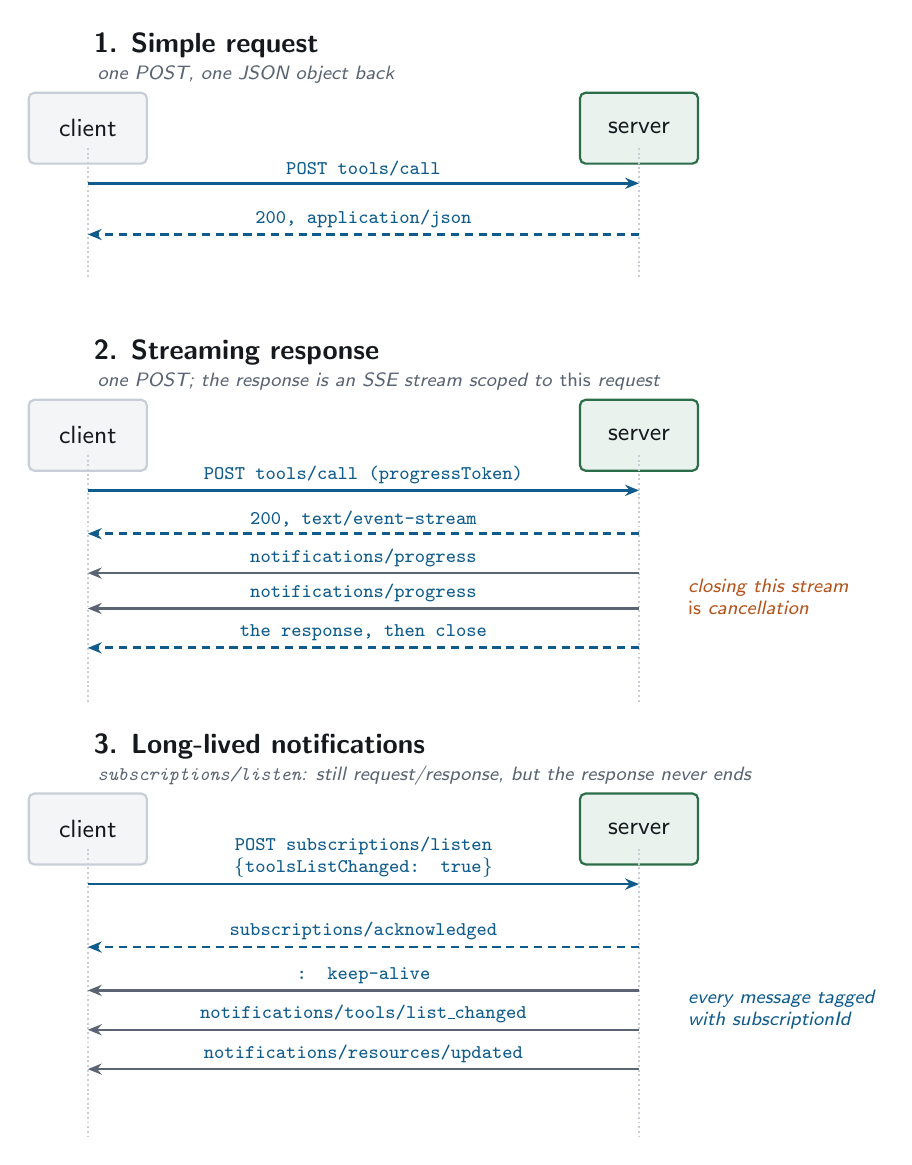
\begin{tikzpicture}[x=1cm, y=1cm]

\def\lane{7.0}

% =========================================================================
\begin{scope}[yshift=0cm]
  \node[lblink, font=\sffamily\bfseries, anchor=west] at (0,2.05) {1. Simple request};
  \node[note, anchor=west] at (0,1.68) {one POST, one JSON object back};
  \node[box, minimum width=15mm] (c1) at (0,1.0) {client};
  \node[boxg, minimum width=15mm] (s1) at (\lane,1.0) {server};
  \draw[lifeline] (0,0.75) -- (0,-0.9);
  \draw[lifeline] (\lane,0.75) -- (\lane,-0.9);

  \draw[flow] (0,0.3) -- node[tag, above] {POST tools/call} (\lane,0.3);
  \draw[flow, densely dashed] (\lane,-0.35)
        -- node[tag, above] {200, application/json} (0,-0.35);
\end{scope}

% =========================================================================
\begin{scope}[yshift=-3.9cm]
  \node[lblink, font=\sffamily\bfseries, anchor=west] at (0,2.05) {2. Streaming response};
  \node[note, anchor=west] at (0,1.68)
    {one POST; the response is an SSE stream scoped to \emph{this} request};
  \node[box, minimum width=15mm] (c2) at (0,1.0) {client};
  \node[boxg, minimum width=15mm] (s2) at (\lane,1.0) {server};
  \draw[lifeline] (0,0.75) -- (0,-2.4);
  \draw[lifeline] (\lane,0.75) -- (\lane,-2.4);

  \draw[flow] (0,0.3) -- node[tag, above] {POST tools/call (progressToken)} (\lane,0.3);
  \draw[flow, densely dashed] (\lane,-0.25)
        -- node[tag, above] {200, text/event-stream} (0,-0.25);
  \draw[flowmuted] (\lane,-0.75)
        -- node[tag, above] {notifications/progress} (0,-0.75);
  \draw[flowmuted] (\lane,-1.2)
        -- node[tag, above] {notifications/progress} (0,-1.2);
  \draw[flow, densely dashed] (\lane,-1.7)
        -- node[tag, above] {the response, then close} (0,-1.7);

  \node[note, anchor=west, text=warm, align=left] at (\lane+0.5,-1.05)
    {closing this stream\\\emph{is} cancellation};
\end{scope}

% =========================================================================
\begin{scope}[yshift=-8.9cm]
  \node[lblink, font=\sffamily\bfseries, anchor=west] at (0,2.05)
    {3. Long-lived notifications};
  \node[note, anchor=west] at (0,1.68)
    {\texttt{subscriptions/listen}: still request/response, but the response never ends};
  \node[box, minimum width=15mm] (c3) at (0,1.0) {client};
  \node[boxg, minimum width=15mm] (s3) at (\lane,1.0) {server};
  \draw[lifeline] (0,0.75) -- (0,-2.9);
  \draw[lifeline] (\lane,0.75) -- (\lane,-2.9);

  \draw[flow] (0,0.3) -- node[tag, above, align=center]
    {POST subscriptions/listen\\\scriptsize\{toolsListChanged: true\}} (\lane,0.3);
  \draw[flow, densely dashed] (\lane,-0.5)
        -- node[tag, above] {subscriptions/acknowledged} (0,-0.5);
  \draw[flowmuted] (\lane,-1.05) -- node[tag, above] {\ttfamily :\ \ keep-alive} (0,-1.05);
  \draw[flowmuted] (\lane,-1.55)
        -- node[tag, above] {notifications/tools/list\_changed} (0,-1.55);
  \draw[flowmuted] (\lane,-2.05)
        -- node[tag, above] {notifications/resources/updated} (0,-2.05);

  \node[note, anchor=west, text=accent, align=left] at (\lane+0.5,-1.3)
    {every message tagged\\with subscriptionId};
\end{scope}

\end{tikzpicture}
\end{document}
